\documentclass{beamer}
\usetheme{metropolis}
\metroset{sectionpage=none}
\definecolor{TUGreen}{rgb}{0.517,0.721,0.094}
\setbeamercolor{background canvas}{bg=white,fg=black}
\setbeamercolor{frametitle}{bg=white,fg=TUGreen}
\setbeamercolor{alerted text}{fg=TUGreen}
\setbeamerfont{bibliography item}{size=\tiny}
\setbeamerfont{bibliography entry author}{size=\tiny}
\setbeamerfont{bibliography entry title}{size=\tiny}
\setbeamerfont{bibliography entry location}{size=\tiny}
\setbeamerfont{bibliography entry note}{size=\tiny}

\makeatletter
\newcommand*{\currentname}{\@currentlabelname}
\setbeamertemplate{footline}[frame number]{}
\setbeamertemplate{frametitle}{%
	\nointerlineskip%
	\begin{beamercolorbox}[%
		wd=\paperwidth,%
		sep=0pt,%
		leftskip=\metropolis@frametitle@padding,%
		rightskip=\metropolis@frametitle@padding,%
		]{frametitle}%
		\begin{minipage}[t]{42ex}
			\metropolis@frametitlestrut@start%
			\insertframetitle%
			\nolinebreak%
			\metropolis@frametitlestrut@end%
		\end{minipage}
		\hfill
		\begin{minipage}[t]{14ex}
			\vspace{-1.6ex}
			
\includegraphics[height=2.2ex,keepaspectratio]{tud_logo_rgb}
		\end{minipage}
	\end{beamercolorbox}%
}
\makeatother

\title{Segmentierung der Marsoberfläche mit Hilfe von unüberwachtem tiefen Clustering}
\subtitle{Bachelorarbeit Abschlusspräsentation}
\author{Max Mustermann}
\date{\today}
\institute[TU Dortmund]{Mustererkennung,\\ Informatik XII, Technische Universität Dortmund}

\begin{document}
\maketitle

\begin{frame}{Inhalt}
\tableofcontents
\end{frame}


\section{Motivation}
\begin{frame}{Motivation: Neuronale Netze zur Bildsegmentierung}
\begin{itemize}
	\item Neuronale Netzwerke werden oft zur Bildsegmentierung genutzt
	\item Gewöhnlich als Voraussetzung: Vorhandene Ground Truth
\end{itemize}% TODO Bild
\end{frame}

\begin{frame}{Motivation: (Fehlende) Ground Truths}
\begin{itemize}
	\item Ground Truths sind nicht immer vorhanden
	\item Beispiel: Marsoberfläche
	\begin{itemize}
		\item Zu großer Datensatz
		\item Notwendigkeit von Domänenexperten
	\end{itemize}
	\item Lösungsansatz:
	\begin{itemize}
		\item Anfangs zufällige Klassifizierung durch Segmentierungsalgorithmus weiter optimieren
	\end{itemize}
\end{itemize}
\end{frame}

%\section{Grundlagen}

\section{Verwandte Arbeiten}



\begin{frame}{Verwandte Arbeiten: Unsupervised Deep Embedding for Clustering Analysis \cite{junyuan_16}}
\begin{itemize}
	\item Unüberwachtes Lernen der Segmentierung
	\item Farbwerte werden zuerst durch $f_\theta:X\rightarrow Z$ (nichtlinear) in Merkmalsraum abgebildet
	\begin{itemize}
		\item $\theta$ ist lernbar
		\item Das NN optimiert $theta$ und Positionen der Clustermitten $\mu_j$¸
	\end{itemize}
\end{itemize}
\end{frame}

\begin{frame}[allowframebreaks]{Verwandte Arbeiten: Segmentierung nach Kanezaki \cite{kanezaki_18}}
	\begin{itemize}
		\item Unüberwachtes Lernen der Segmentierung
		\item Vergleichbar mit, aber einfacher als DEC
		\item Anfangs zufällige Ergebnisse werden mit Clusteringalgorithmus (hier SLIC \cite{achanta_10} vereint)
		\item Verlustfunktion: Cross-Entropy-Loss zwischen Ergebnis des NN und des verfeinerten Ergebnisses
		\item NN wird durch Backpropagation auf diese Zielfunktion hin optimiert
	\end{itemize}
	\begin{figure}
		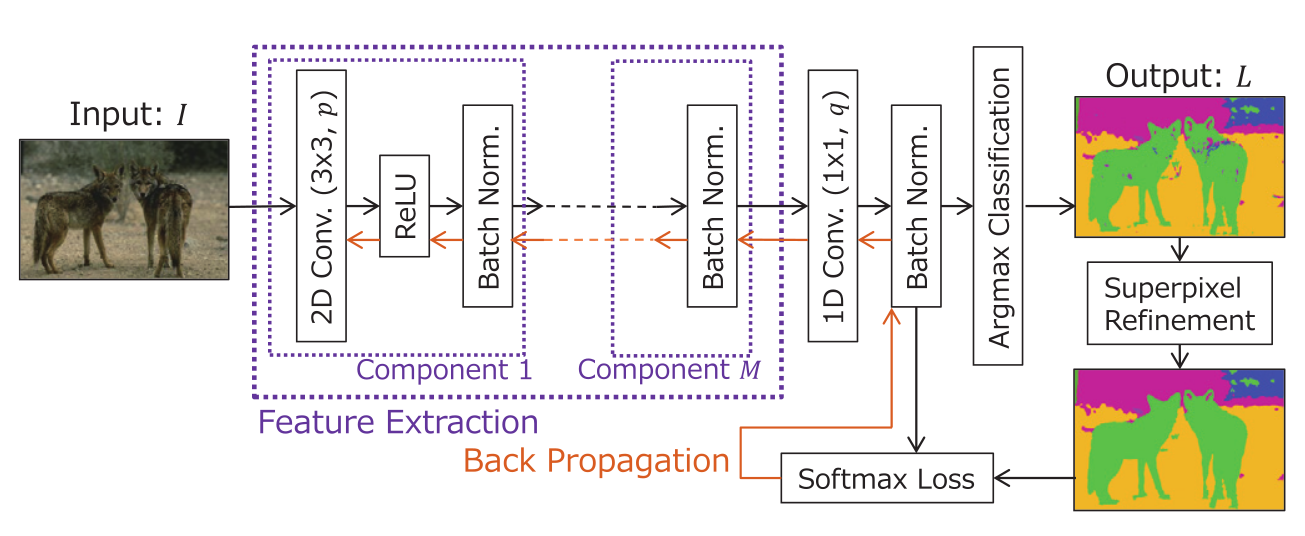
\includegraphics[height=20ex,keepaspectratio]{gfx/Kan18_01.png}
	\end{figure}
\end{frame}

\section{Methodik}



\section{Resultate}



\begin{frame}[allowframebreaks]{Referenzen}
	\setbeamertemplate{bibliography item}[text]
	\bibliographystyle{alpha}
	\bibliography{literatur}
\end{frame}
\end{document}